\pagenumbering{arabic}
\phantomsection\section*{\centering CHƯƠNG 1.	CÁC QUI ĐỊNH CHUNG}
\addcontentsline{toc}{section}{\numberline{}CHƯƠNG 1. CÁC QUI ĐỊNH CHUNG}
\setcounter{section}{1}
\setcounter{subsection}{0}
\setcounter{figure}{0}
\setcounter{table}{0}
Phần mở đầu giới thiệu vấn đề mà đồ án cần giải quyết mô tả được các phương pháp hiện có để giải quyết vấn đề, trình bày mục đích của đồ án song song với việc giới hạn phạm vi của vấn đề mà đồ án tập chung giải quyết. Phần này cũng giới thiệu tóm tắt cấu trúc đồ án và nội dung tương ứng của các phần sẽ lần lượt được trình bày ở các chương tiếp theo.

Nội dung chính của 1 đồ án tốt nghiệp bao gồm:
\begin{itemize}
    \item Phần mở đầu giới thiệu đề tài.
    \item Một chương giới thiệu cơ sở lý thuyết.
    \item Một hoặc nhiều chương trình bày các vấn đề về tính toán và thiết kế.
    \item Một chương mô tả các thí nghiệm và kết quả thu được.
\end{itemize}


\cleardoublepage
\phantomsection\section*{\centering CHƯƠNG 2. SỬ DỤNG CÁC BIỂU ĐỒ}
\addcontentsline{toc}{section}{\numberline{}CHƯƠNG 2. SỬ DỤNG CÁC BIỂU ĐỒ}
\setcounter{section}{2}
\setcounter{subsection}{0}
\setcounter{figure}{0}
\setcounter{table}{0}
Mỗi chương sẽ bắt đầu bằng đoạn giới thiệu các phần chính được trình bày trong chương đó, dài khoảng 5 - 10 dòng và kết thúc bằng 1 đoạn tóm tắt các kết luận chính của chương. Chú ý phân bổ chiều dài của mỗi chương cho cân đối và hợp lý 
\subsection{Một số lưu ý khi trình bày đồ án}
Sau đây là 1 vài chú ý khi làm đồ án các bạn cần nhớ nhé
\subsubsection{Nộp đồ án}
Sinh viên (hoặc nhóm sinh viên tối đa 3 thành viên làm chung 1 đề tài) phải nộp 2 quyển đồ án tốt nghiệp tại văn phòng bộ môn của giảng viên hướng dẫn trước ngày bảo vệ ít nhất 1 tuần. Một quyển đồ án cần có các đặc điểm sau:
\begin{itemize}
    \item Được \textbf{in 2 mặt} nhằm tiết kiệm không gian lưu trữ.
    \item Đóng bìa mềm, bên ngoài là bóng kính. 
    \item Số trang 50 - 150 trang, không kể phần phục lục
    \item Phải có chữ ký của sinh viên sau lời cam đoan và của giảng viên hướng dẫn. 
\end{itemize}
\subsubsection{Phụ lục}
Phụ lục nếu có chứa thông tin có liên quan đến đồ án nhưng nếu để trong phần chính sẽ gây rườm rà. Thông thường các chi tiết để trong phần phụ lục là kết quả thô (chưa qua xử lý), mã nguồn phần mềm, thông số chi tiết của linh kiện hoặc hình thành minh họa thêm...
\subsubsection{Tài liệu tham khảo}
\paragraph{Cách liệt kê} \mbox{} % mbox để xuống dòng 

Áp dụng cách liệt kê theo quy định của IEEE. Theo đó tài liệu tham khảo được đánh số thứ tự trong ngoặc vuông. Thứ tự liệt kê là thứ tự xuất hiện của tài liệu tham khảo được trích dẫn trong đồ án. Tài liệu tham khảo đã liệt kê bắt buộc phải được trích dẫn trong phần nội dung của đồ án. Tài liệu tham khảo cần có nguồn gốc rõ ràng và phải từ nguồn đáng tin cậy. Cần hạn chế trích dẫn tài liệu tham khảo từ các website, từ wikipedia.
\paragraph{Các loại tài liệu tham khảo} \mbox{} % mbox để xuống dòng 

Các nguồn tài liệu tham khảo chính là sách, bài báo trong các tạp chí, bài báo trong các hội nghị khoa học và các tài liệu tham khảo khác trên internet.
\subsubsection{Đánh số phương trình}
Phương trình được đánh số theo số của chương, như hình vẽ và bảng biểu.
\subsubsection{Đánh số định nghĩa, định lý, hệ quả}
Các định nghĩa định lý hệ quả sẽ được đánh số theo số của chương và được sử dụng chung 1 chỉ số. Ví dụ trong chương 3, các định nghĩa, định lý, hệ quả sẽ được đánh số theo thứ tự: Định lý 3.1 , Định nghĩa 3.2, Hệ quả 3.3, Định lý 3.4...

\cleardoublepage
\phantomsection\section*{\centering CHƯƠNG 3. THUẬT TOÁN}
\addcontentsline{toc}{section}{\numberline{}CHƯƠNG 3. THUẬT TOÁN}
\setcounter{section}{3}
\setcounter{subsection}{0}
\setcounter{figure}{0}
\setcounter{table}{0}
Đây \cite{stein2011fourier} là phần sinh viên tự phát triển như xây dựng thuật toán, xây dựng chương trình, mô phỏng, tính toán, thiết kế, chạy thử kết quả... \cite{howell2016principles}
\subsection{Cách chèn ảnh}
\begin{figure}[H]
    \centering
    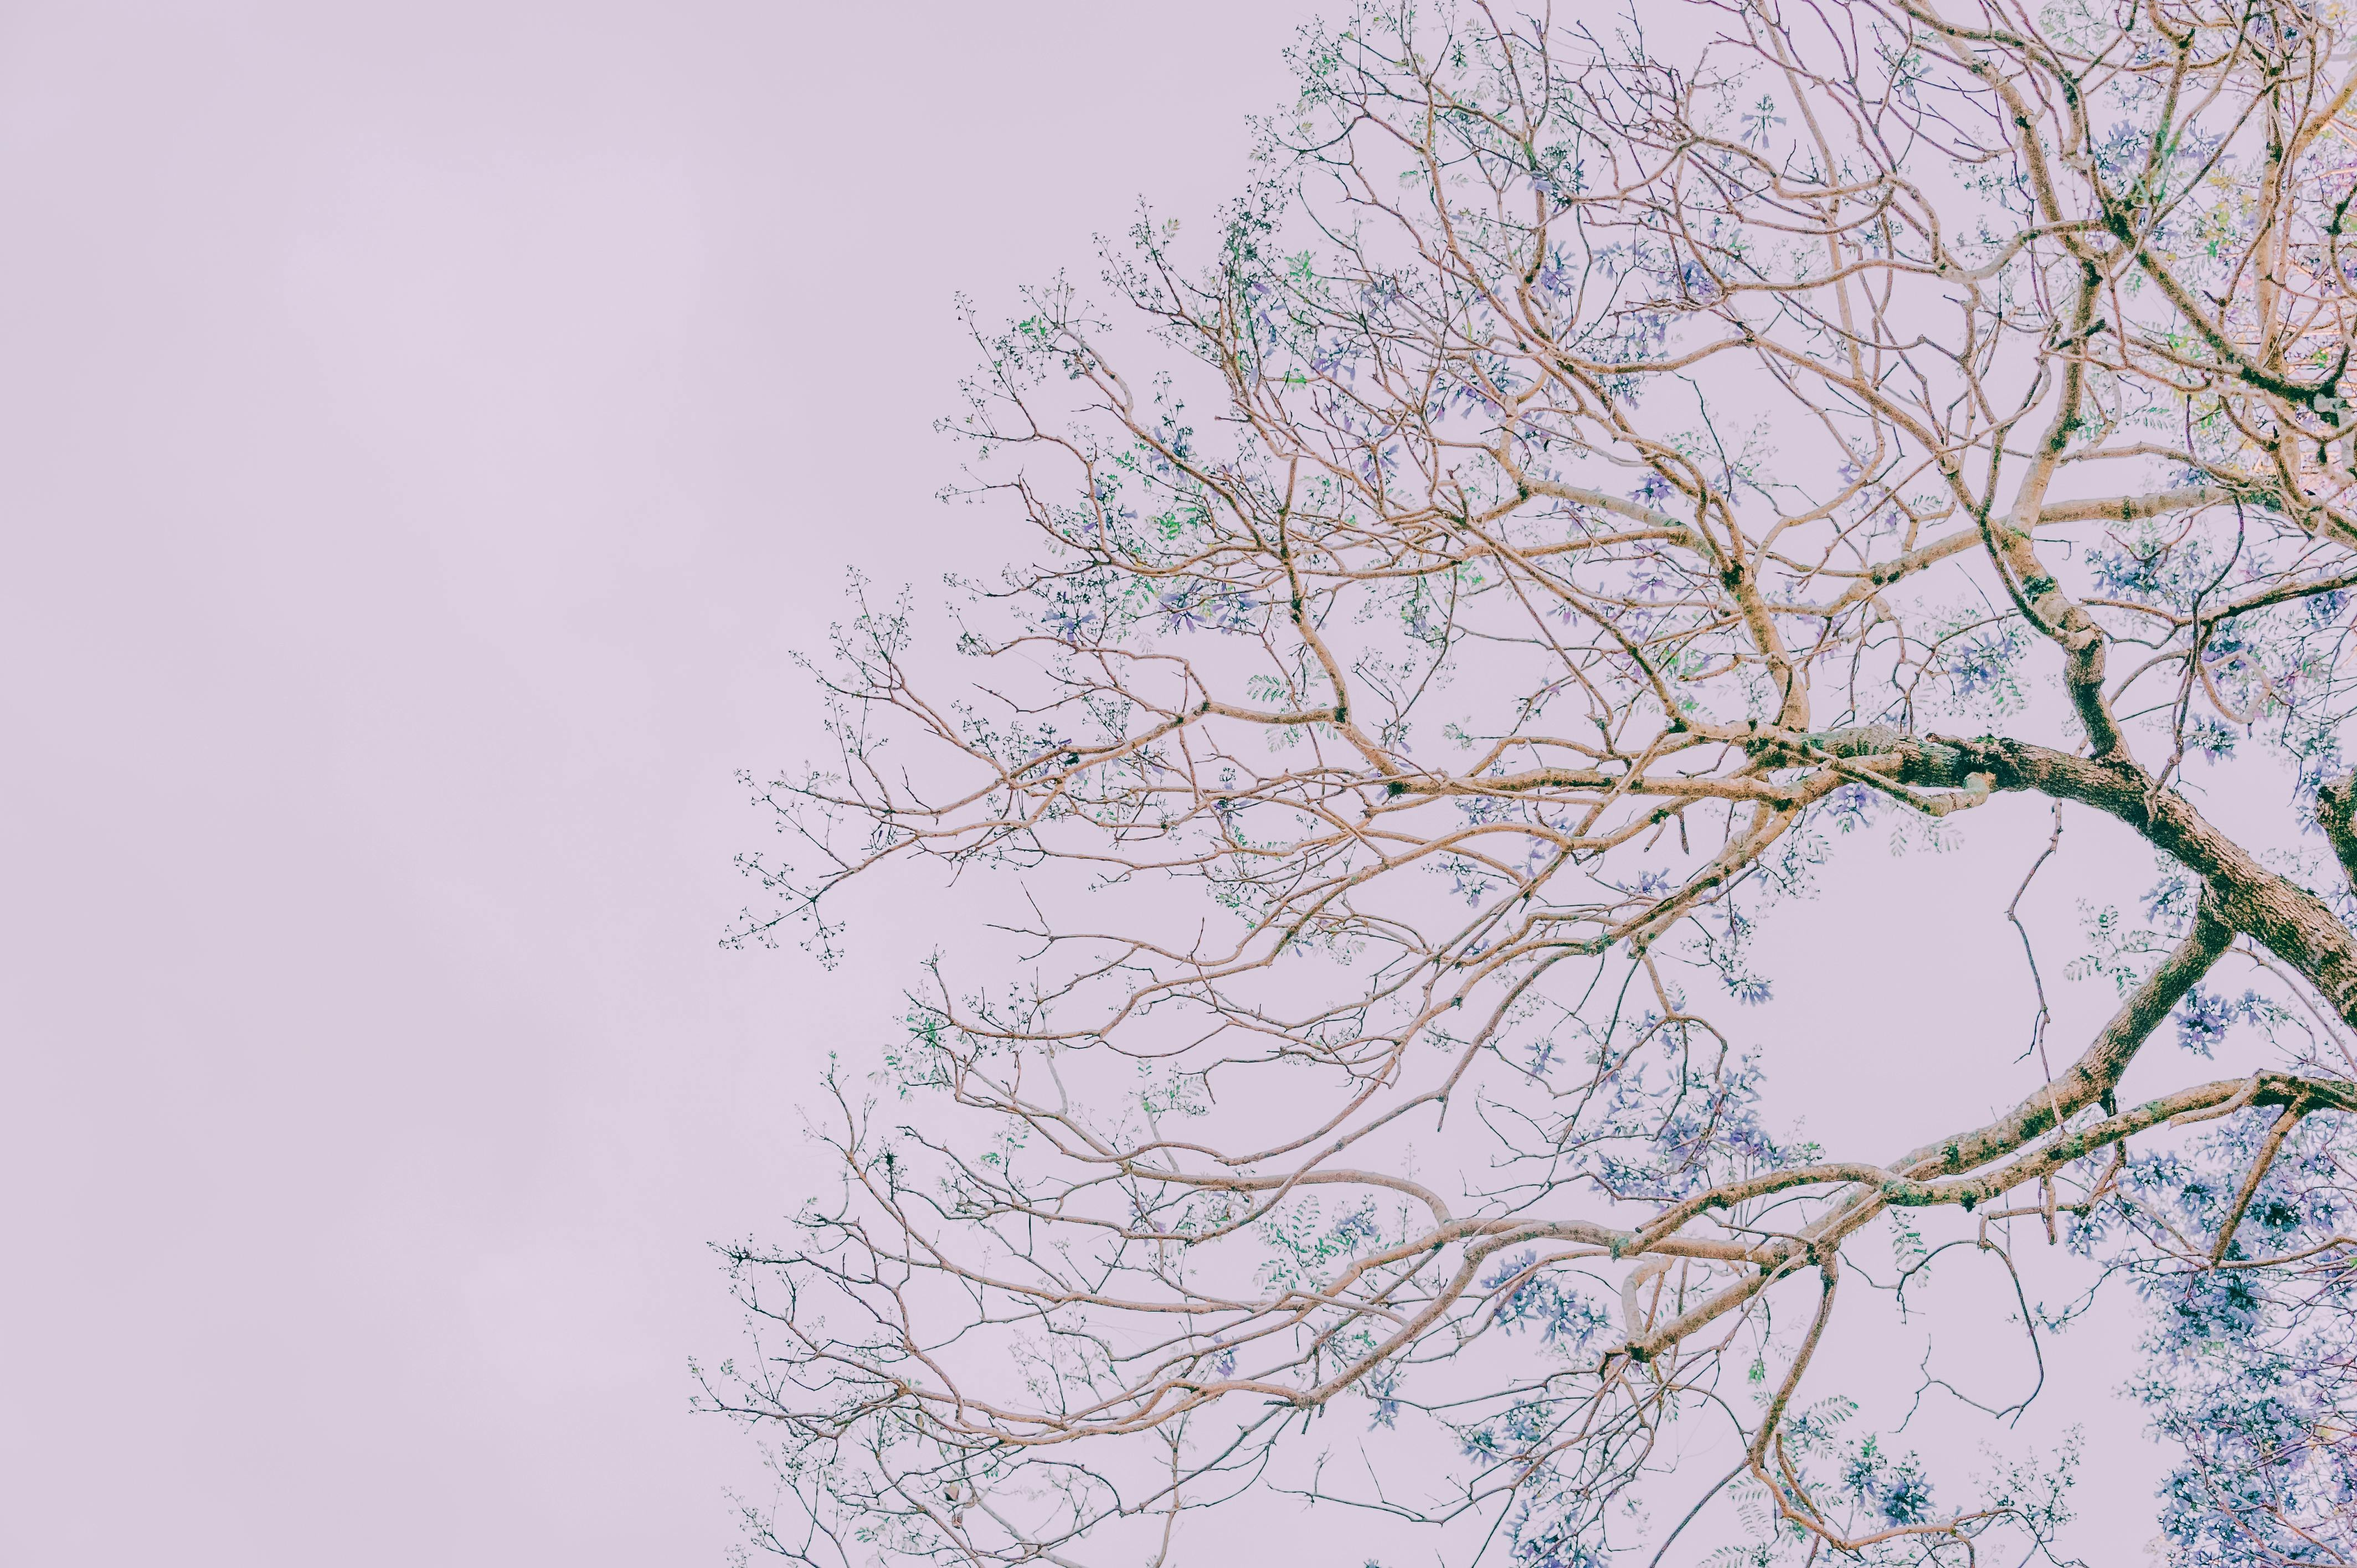
\includegraphics[width=0.75\textwidth, height=4.39cm]{image/Tree.jpg}
    \caption[Sơ đồ khối của hệ thống]{\textit{\fontsize{12pt}{0}\selectfont Sơ đồ khối của hệ thống}}
    \label{hinh31}
\end{figure}
Hình \ref{hinh31} là ví dụ về cách chèn ảnh. Lưu ý chú thích của hình vẽ được đặt ngay dưới hình vẽ. Tất cả các hình vẽ phải được đề cập đến trong phần nội dung và phải được phân tích và bình luận giống mình đang làm thế này nhé hihi :)

\subsection{Cách tạo bảng}
\begin{table}[H]
    \centering
    \caption[Kết quả thí nghiệm]{\textit{\fontsize{12pt}{0}\selectfont Kết quả thí nghiệm}}
    \begin{tabularx}{0.75\textwidth}{
        |>{\centering\arraybackslash}s
        |>{\centering\arraybackslash}a
        |>{\centering\arraybackslash}a
        |>{\centering\arraybackslash}s|
        }
        \hline
        \bfseries Lần thí nghiệm & \bfseries Điện áp đo được (mV) &\bfseries Điện áp tham chiếu (mV)& \bfseries Sai lệch (\%)\\\hline
        1&&&\\\hline
        2&&&\\\hline
        3&&&\\\hline
    \end{tabularx}
    \label{bang31}
\end{table}
Bảng \ref{bang31} là ví dụ về cách tạo bảng. Lưu ý chú thích của bảng được đặt ở trước bảng. Tất cả các bảng biểu phải được đề cập đến trong phần nội dung và phải phân tích và bình luận giống như mình đang làm nhé hehe :)

\subsection{Cách viết phương trình}
\begin{equation}
    \label{pt31}
    F(x) = \int^a_b \frac{1}{3}x^3
\end{equation}
Phương trình \ref{pt31} là ví dụ về phương trình tích phân.

Thử phương trình khác 
\begin{equation}
    \label{pt32}
    x[t_n] = \frac{1}{\sqrt{n}} \sum_{k=0}^{N-1}[f_k]
\end{equation}
Phương trình \ref{pt32} là phương trình biến đổi Fourier
\subsection{Cách viết định nghĩa, định lý, hệ quả, bổ đề...}
Định lý lấy mẫu Nq-shannon là một định lý được sử dụng trong lĩnh vực lý thuyết thông tin đặc biệt là trong viễn thông và xử lý tín hiệu 
\begin{theorem} % Định lý
    \label{dlNq}
    Một hàm số tín hiệu  $x(t_n)$ không chứa bất kỳ thành phần tần số nào lớn hơn hoặc bằng 1 giá trị $f_m$ có thể biểu diễn chính xác bằng tập các giá trị của nó với chu kỳ lấy mẫu $T = 1/(2f_m)$.
\end{theorem}
Định lý \ref{dlNq} thường được gọi đơn giản là định lý lấy mẫu 
\begin{corollary}
    Một người có thể làm được thì sẽ nghĩ mình làm đư
\end{corollary}
\begin{lemma}
    Một người có thể làm được thì sẽ nghĩ mình làm đư
\end{lemma}
\begin{defn}
    \label{defn}
    Một người có thể làm được thì sẽ nghĩ mình làm đư
\end{defn}
Định nghĩa \ref{defn} được nhắc tới như là tiếng gọi hoang rã từ nơi không người
\cleardoublepage

\phantomsection\section*{\centering CHƯƠNG 4. THÍ NGHIỆM VÀ KẾT QUẢ}
\addcontentsline{toc}{section}{\numberline{} CHƯƠNG 4. THÍ NGHIỆM VÀ KẾT QUẢ}
\setcounter{section}{4}
\setcounter{subsection}{0}
\setcounter{figure}{0}
\setcounter{table}{0}
\subsection{Sao nó không đúng?}
\lipsum
\begin{figure}[H]
    \centering
    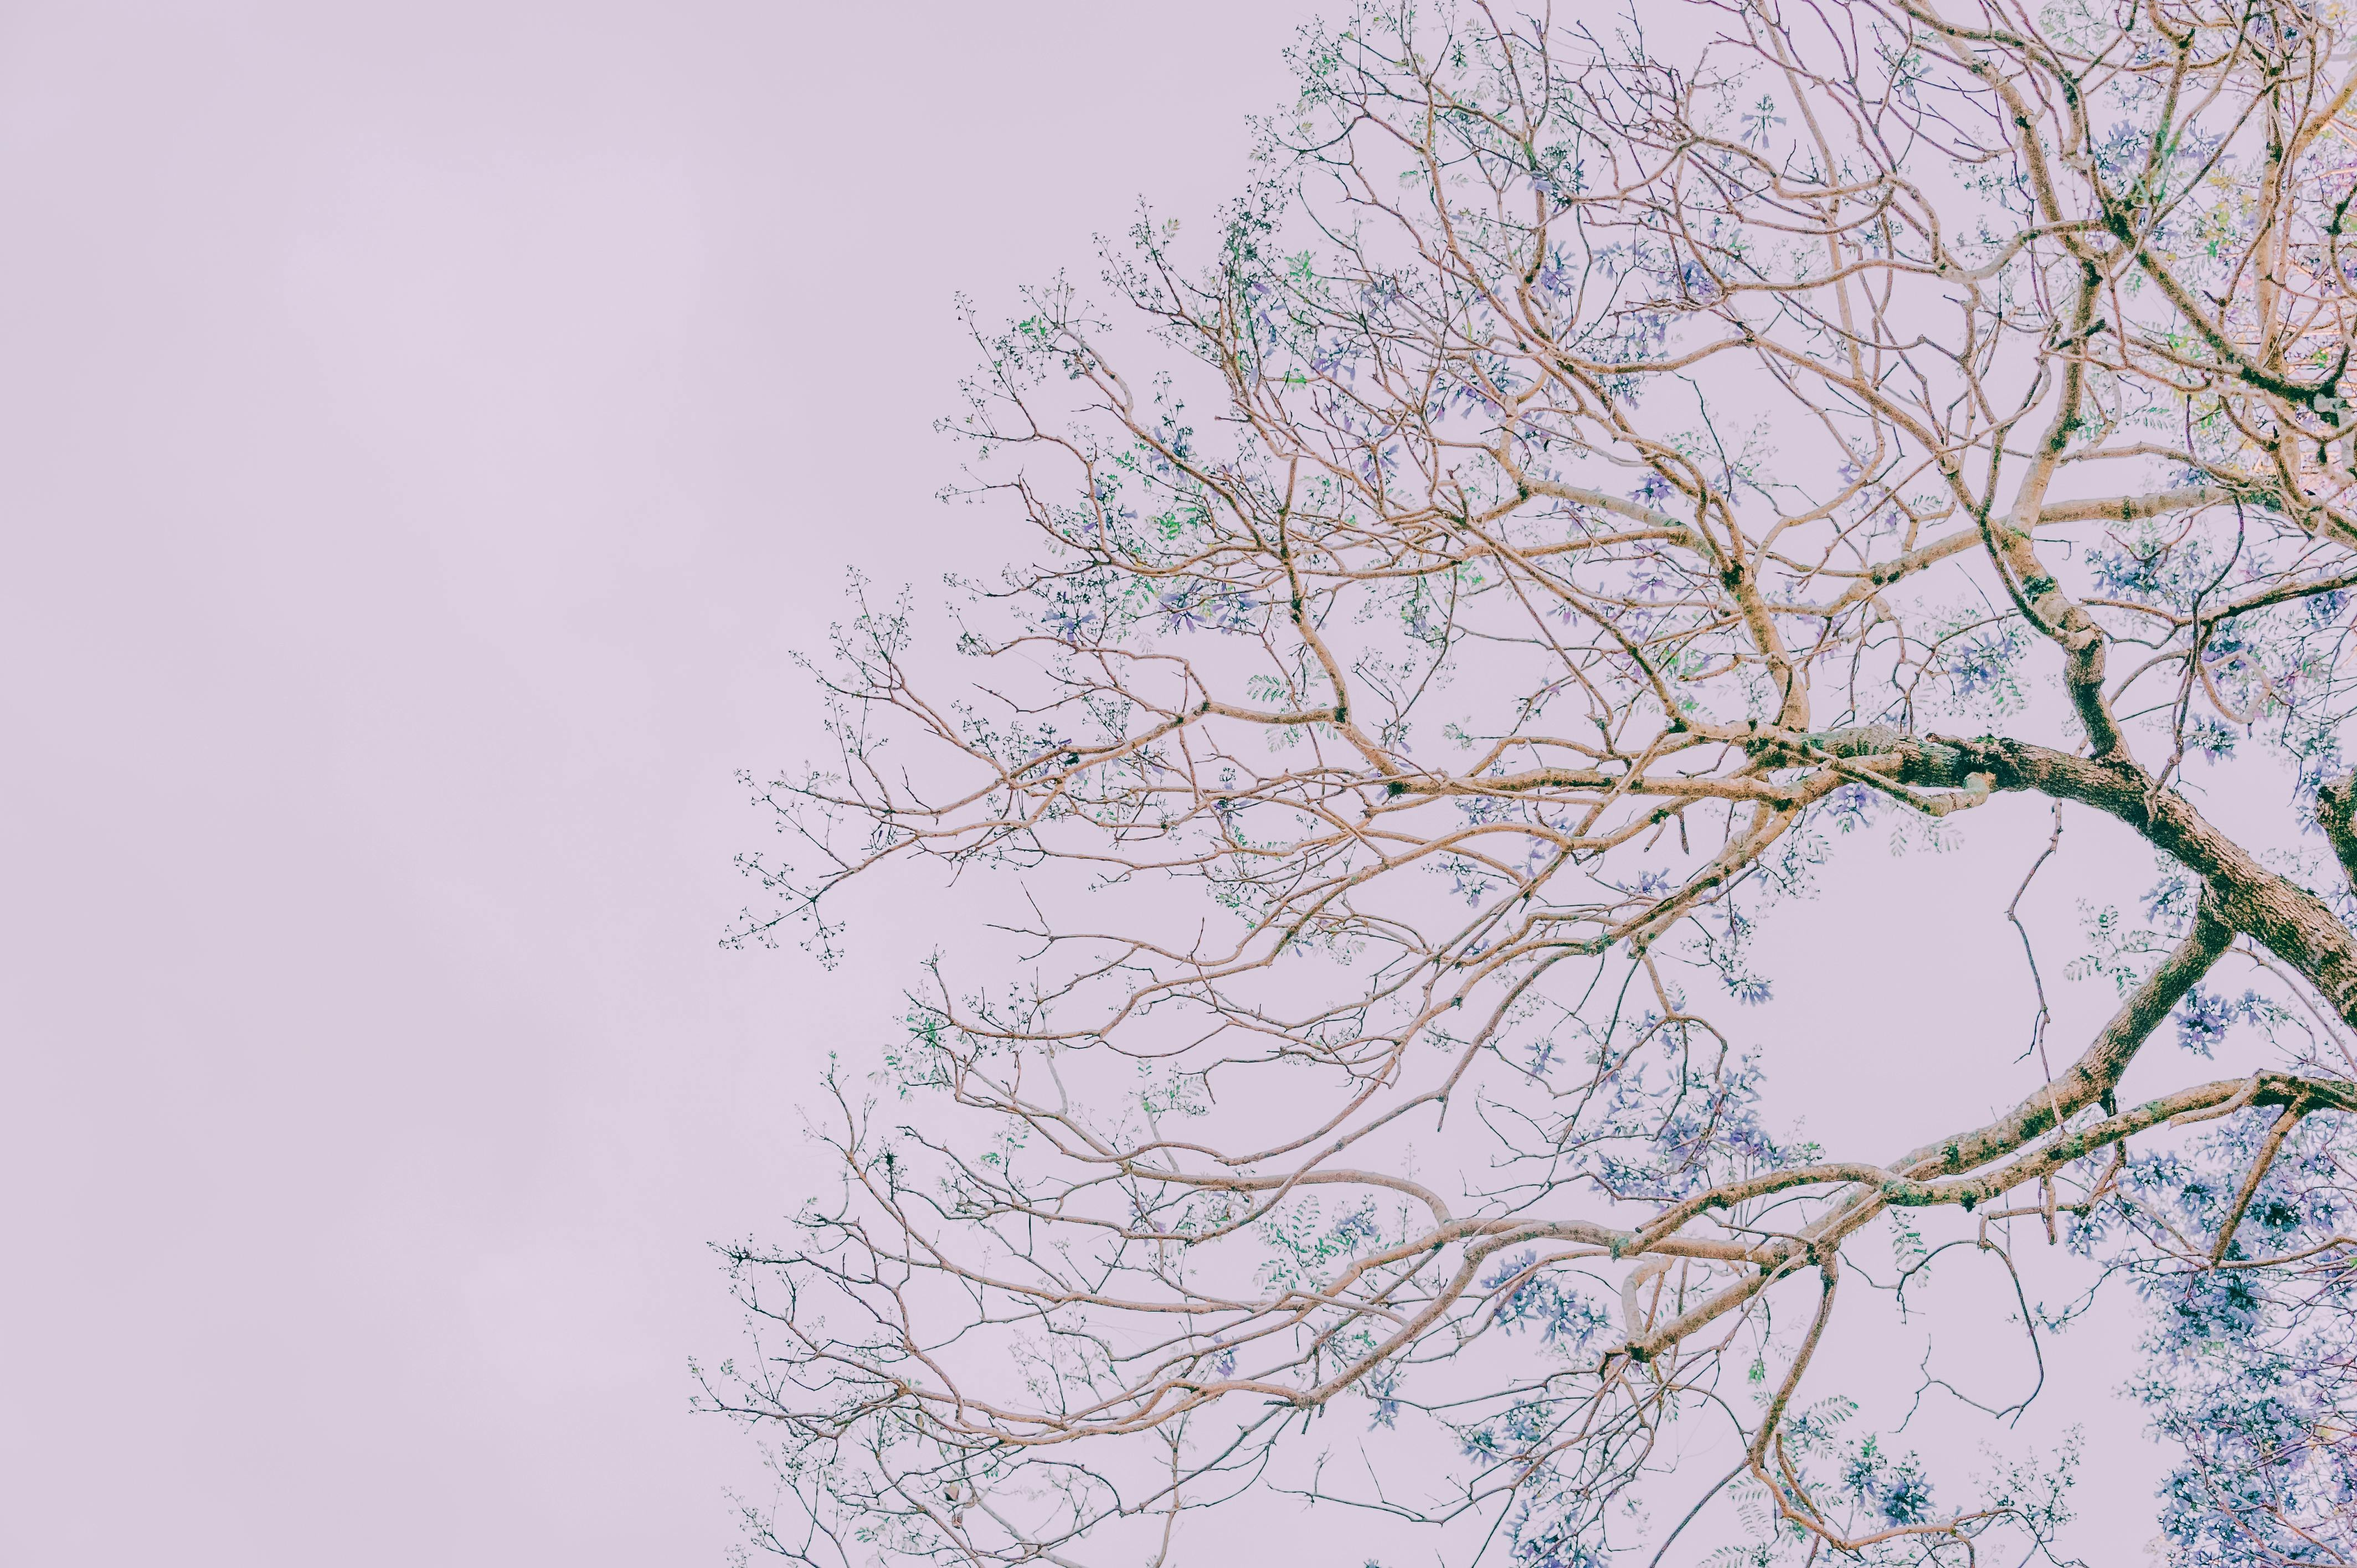
\includegraphics[width=0.75\textwidth, height=4.39cm]{image/Tree.jpg}
    \caption[Sơ đồ khối của hệ thống]{\textit{\fontsize{12pt}{0}\selectfont Sơ đồ khối của hệ thống}}
    \label{hinh4.1}
\end{figure}
Hình \ref{hinh4.1} đây là ví dụ về cách chèn ảnh. Và cách chèn tài liệu tham khảo \cite{bracewell1989fourier}
\cleardoublepage